

%========
% FIGURES 
%========

\newcommand{\FigureOne}{
\begin{figure}
\centering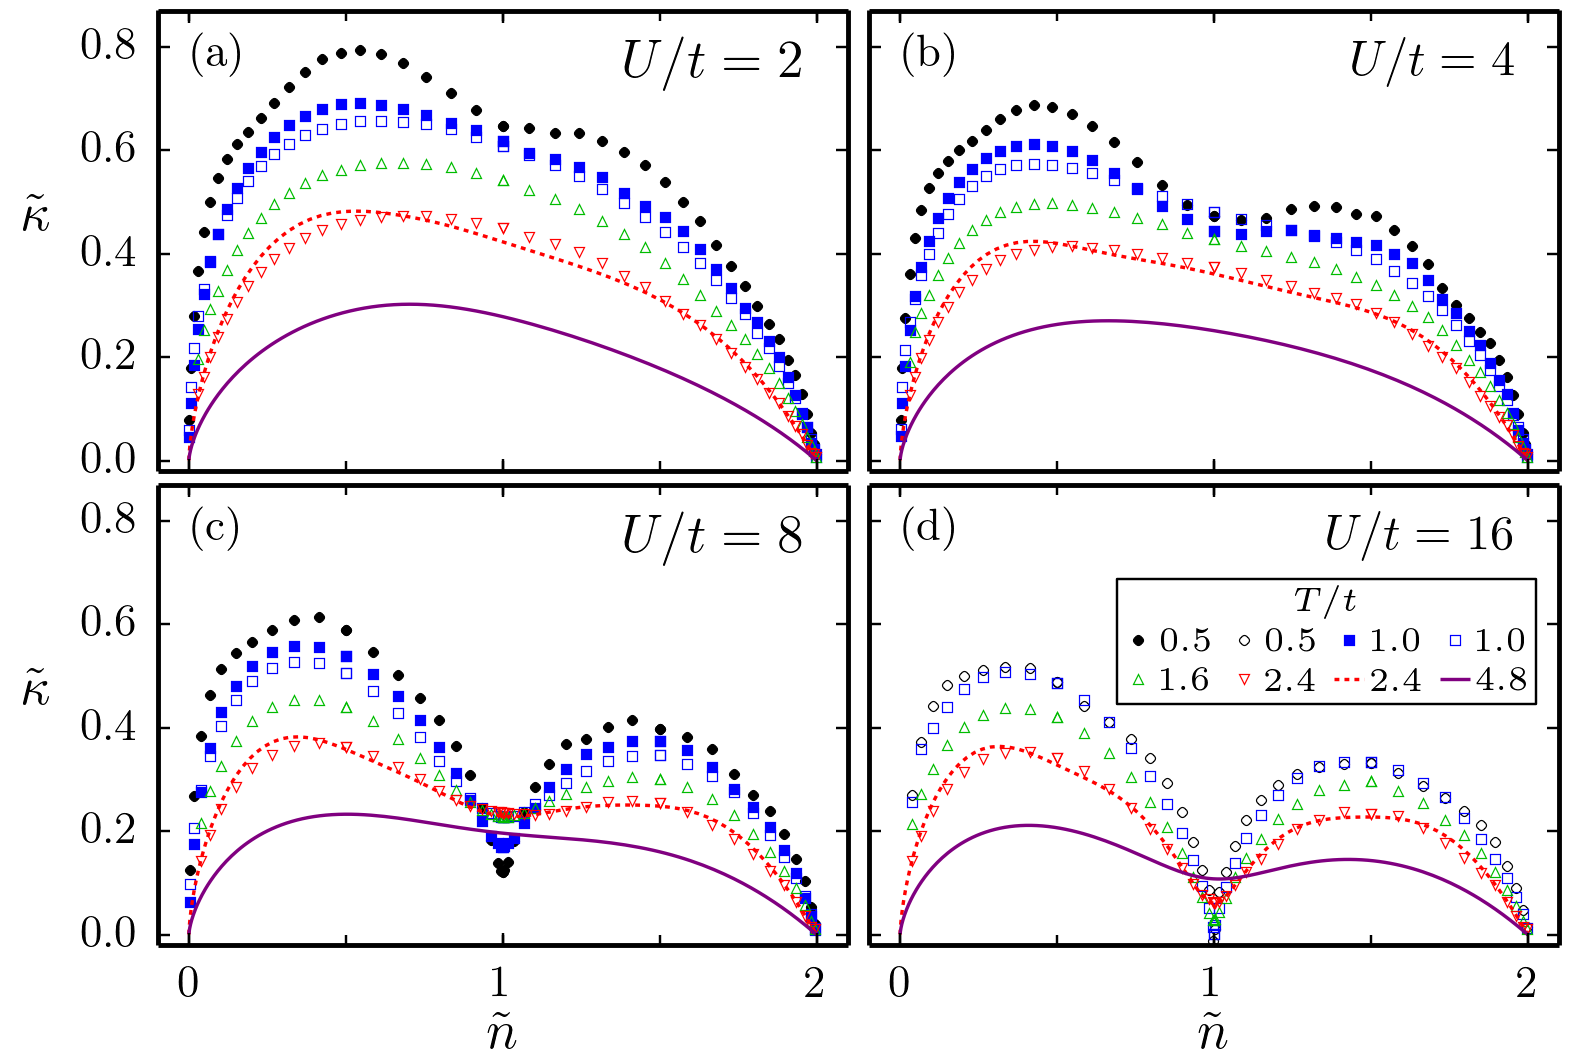
\includegraphics[width=\columnwidth]{../figures/ins/Fig1.png}
\caption{Normalized compressibility versus density for the homogeneous Hubbard
model in three dimensions, shown for various interaction strengths and
temperatures.  The different curves were obtained using DQMC (closed symbols)
NLCE (open symbols)  and the second order HTSE (lines). At half-filling,
$\tilde{n}=1$, the compressibility vanishes for strong interactions and low
temperatures as the system enters the Mott insulating regime.  }
\label{fig:fig1}
\end{figure}
}

\newcommand{\FigureTwo}{
\begin{figure}
\centering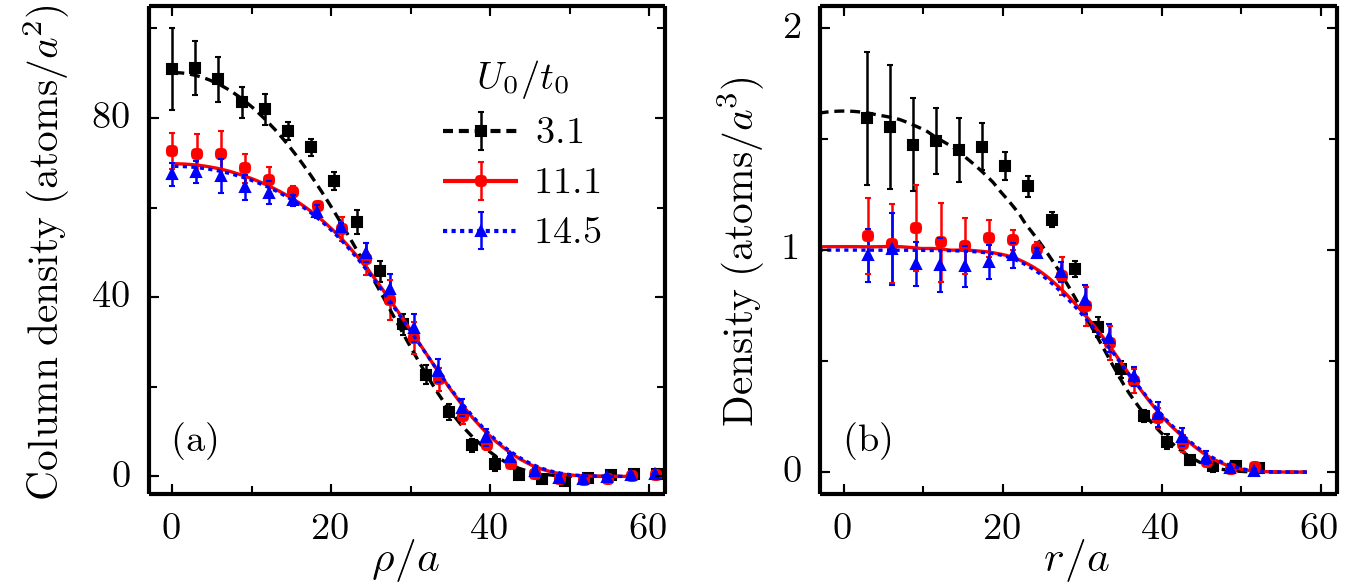
\includegraphics[width=\columnwidth]{../figures/ins/Fig2.png} %
\caption{(a) Azimuthally averaged column density (includes both
spin states) vs. distance from the imaging axis $\rho$, for different values of
$U_{0}/t_{0}$.  Data points represent the average of eight individual
realizations, with error bars corresponding to the standard deviation.  The
lines in (a) are obtained by integrating the density, calculated for
$N=2\times10^{5}$ atoms at $T/t_{0}=0.6$, along the imaging axis.  (b) Data
points correspond to density profiles extracted from the column densities using
the inverse Abel transform, where $r$ is the distance from the center of the
trap.  The lines in (b) show the density calculated for our trap along a body
diagonal of the lattice.  }	
%The inverse Abel transform is applied to the azimuthal average for each of the
%eight realizations (spherical symmetry is assumed), and the results are
%averaged (closed symbols), with error bars corresponding to the standard
%deviation. 
\label{fig:mottfig2}	
\end{figure}
}


\newcommand{\FigureThree}{
\begin{figure}
\centering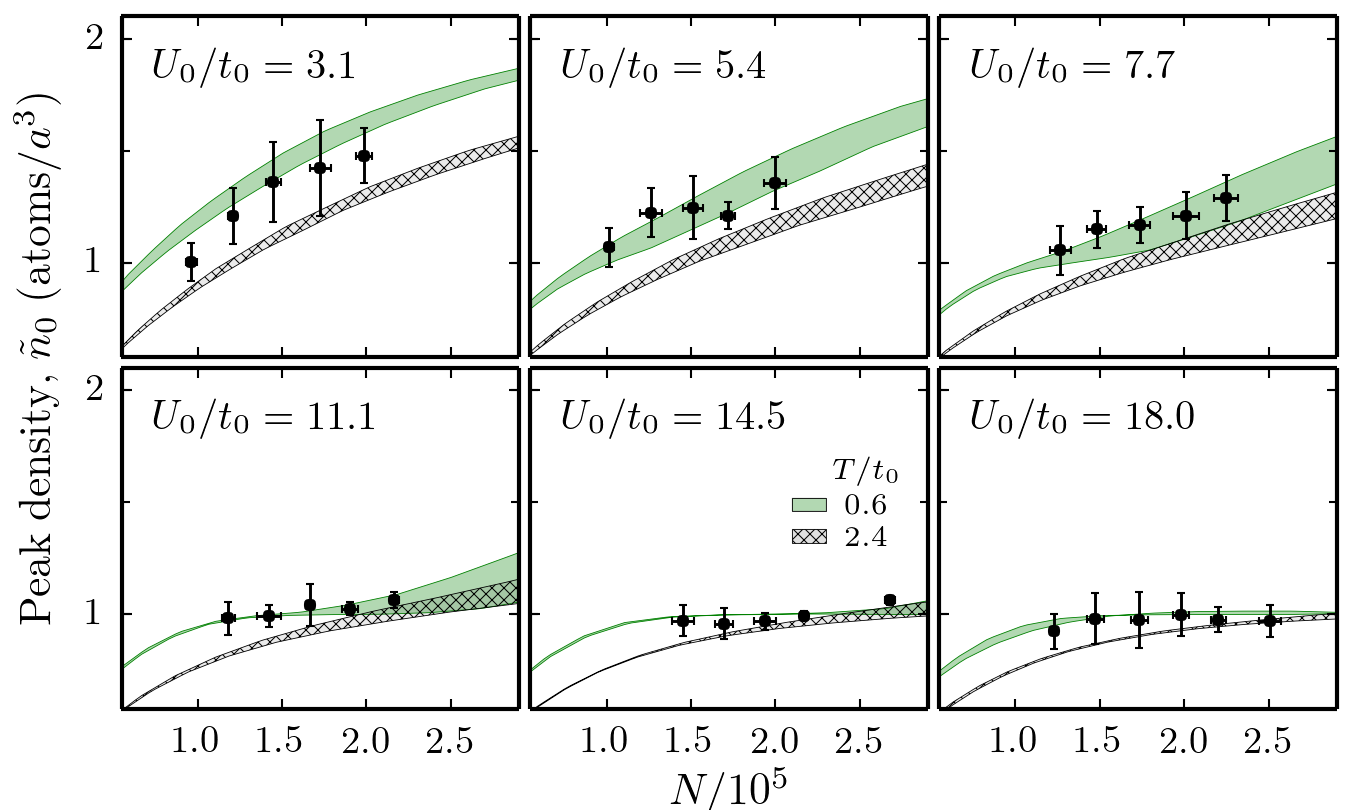
\includegraphics[width=\columnwidth]{../figures/ins/Fig3.png} \caption{ Peak
density, $\tilde{n}_{0}$ vs. atom number for various interaction strengths.  A
fit to the column density of the cloud is used to obtain $\tilde{n}_{0}$.  The
symbols show the average for a set of 5 to 10 independent realizations, with
error bars indicating the standard deviation.  The shaded regions are numerical
calculations for our trap at $T/t_{0}=0.6$ and 2.4, with the width of the
region corresponding to a $\pm14$\% uncertainty in the value of $U_{0}/t_{0}$.
}
\label{fig:n0mott}
\end{figure}
}

\newcommand{\FigureFour}{
\begin{figure}
\centering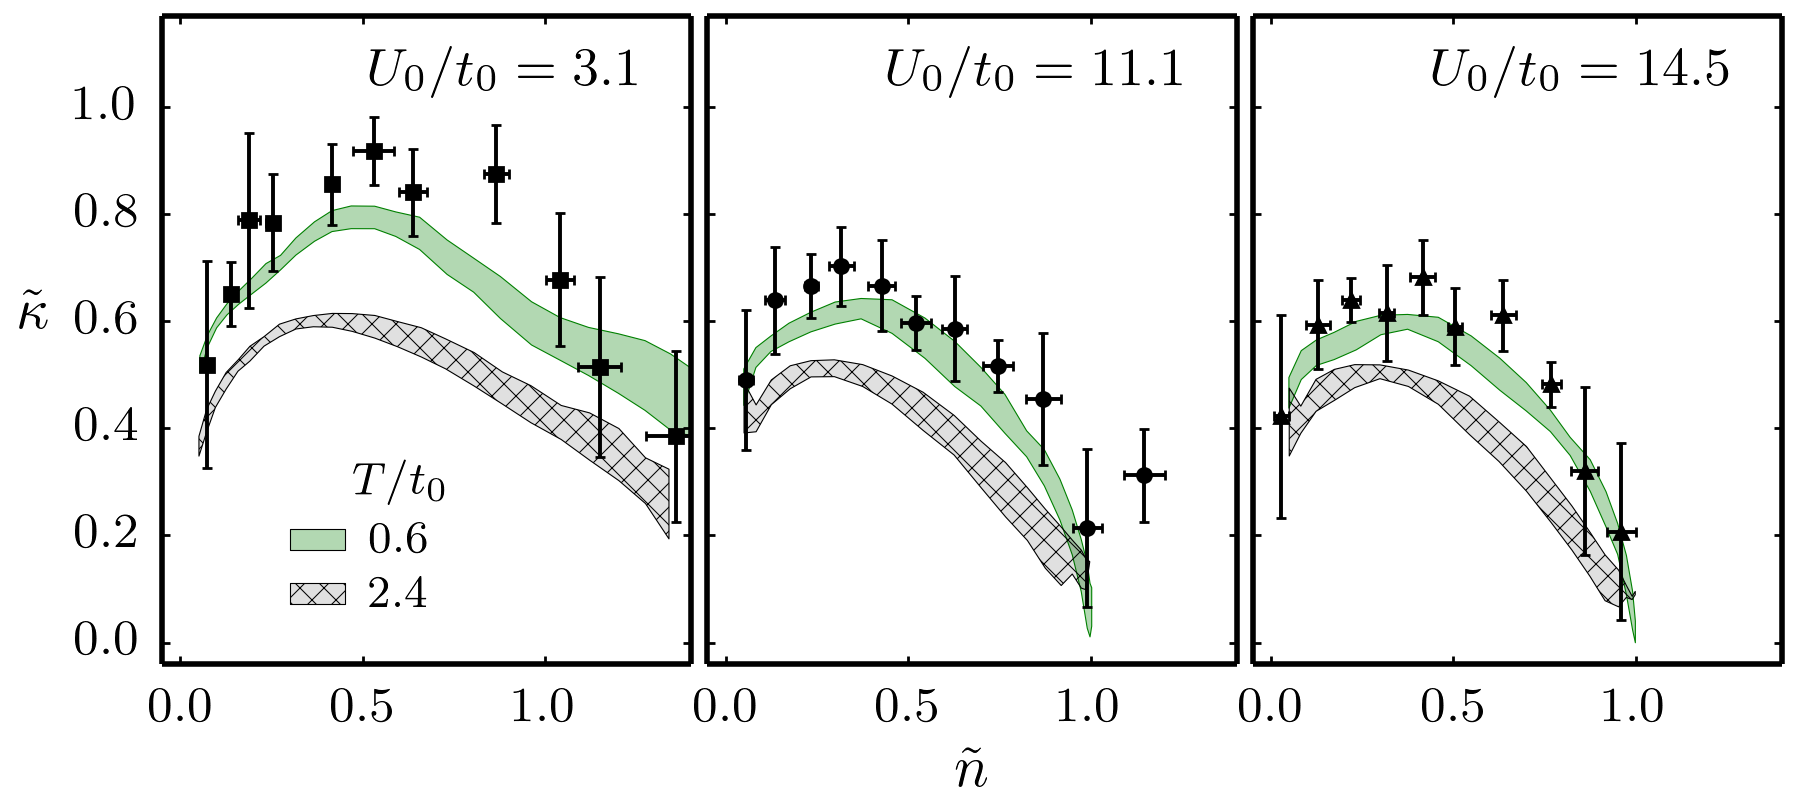
\includegraphics[width=\columnwidth]{../figures/ins/Fig4.png}
\caption{Normalized compressibility, $\tilde{\kappa}$ versus
density for different values of $U_{0}/t_{0}$.  Closed symbols show the average
of eight individual realizations with error bars indicating the standard
deviation.  The shaded regions are numerical calculations at $T/t=0.6$ and
$T/t=2.4$f or $N=2\times 10^{5}$,
where the width of the region reflects a $\pm$14\% systematic uncertainty in
$U_{0}/t_{0}$.}
\label{fig:compr-mott}
\end{figure}
}

%%%%%%%%%%%%%%%%%%%%%%%%%%%%%%%%%%%%%%%%%%%%%%%%%%%%%%%%%%%%%%%%%%%%%%%%%%%%%%%
%%%%%%%%%%%%%%%%%%%%%%%%%%%%%%%%%%%%%%%%%%%%%%%%%%%%%%%%%%%%%%%%%%%%%%%%%%%%%%%
%%%%  CHAPTER MOTT 
%%%%%%%%%%%%%%%%%%%%%%%%%%%%%%%%%%%%%%%%%%%%%%%%%%%%%%%%%%%%%%%%%%%%%%%%%%%%%%%
%%%%%%%%%%%%%%%%%%%%%%%%%%%%%%%%%%%%%%%%%%%%%%%%%%%%%%%%%%%%%%%%%%%%%%%%%%%%%%%
\chapter{Mott insulating state in a simple cubic lattice}
\label{chap:mott}

The contents of this chapter are based on a recently submitted paper titled
``Compressibility of a fermionic Mott insulator of ultracold
atoms''~\cite{Duarte2014arxiv}.  

We realize the repulsive Hubbard model in a 7$E_{r}$ lattice.  The scattering
length is adjusted in the range of $80\,a_{0}-470\,a_{0}$, which results in
interaction strengths $U_{0}/t_{0}$ in the range 3.1 to 18.0.  The number of
atoms for this study was varied between 1$\times10^{5}$ and 2.5$\times10^{5}$.
As was mentioned in Chapter~\ref{chap:compensated-optical-lattice},  in our
realization the Hubbard parameters are not constant throughout the extent of
the cloud, so we use the subscript $_{0}$ to indicate the value of the Hubbard
parameters at the center of the sample.

We perform measurements of the \textit{in-situ} column density of the
atom cloud and analyze them to extract quantities that reveal the Mott
insulating regime in a simple cubic lattice with repulsive interactions.
An example of the measured column density distributions is shown in
Fig.~\ref{fig:mott-fit-cloud}. 
\begin{figure}
    \centering
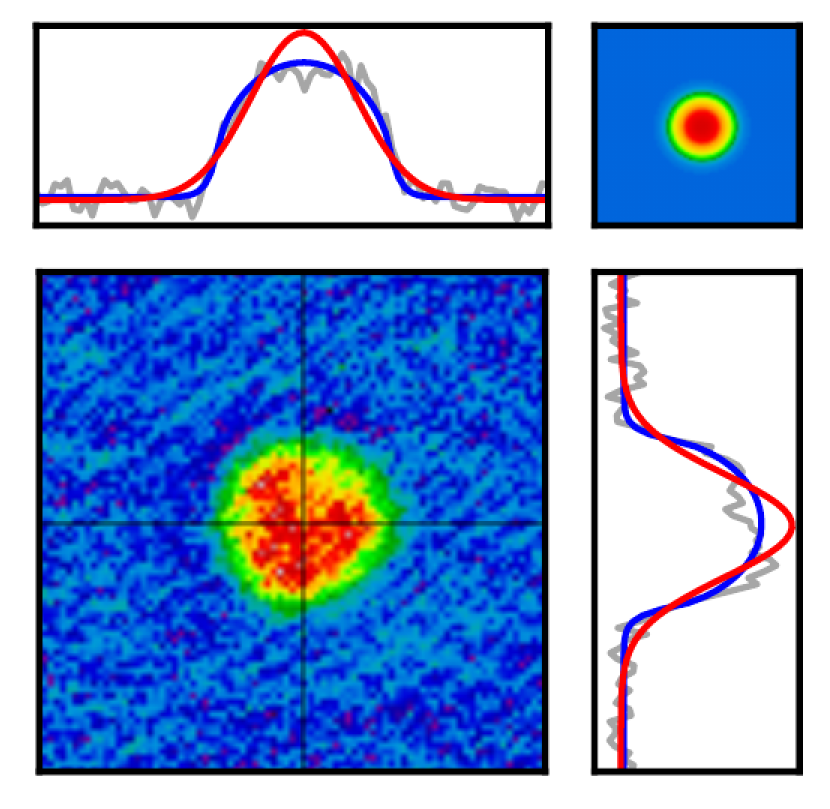
\includegraphics[width=0.4\textwidth]{../figures/mott/mott-fit-cloud.png}
\caption{\small Column density distribution taken in a 7\,$E_{r}$ lattice at a
scattering length $a_{s}=380\,a_{0}$.  The on-site interactions are
$U/t_{0}$=14.5. The lines are fits to the column density
distribution which are explained in the text. }  
\label{fig:mott-fit-cloud}
\end{figure}
A fit to a Gaussian distribution (red line in the figure)  clearly does not
properly describe the column density profile of the cloud.   As was shown in
Chapter~\ref{chap:compensated-optical-lattice}, density profiles calculated
within the local density approximation (LDA) for large interaction strengths
(as the system enters the Mott insulating regime), are expected to have an
$n=1$ Mott insulating plateau at the center.  Guided by the results of the LDA,
we implemented a fit function that can interpolate between a Gaussian fit and
what we call a Mott fit.   The Mott fit function is the column
integral\footnote{ The column integral is defined as  
\begin{equation}
 \tilde{n}_{\mathrm{col}}(\rho) = \int \tilde{n}( \rho, z ) \,\mathrm{d}z , 
\end{equation}}
of a flat-topped density distribution function given by
\begin{equation}
 \tilde{n}(\rho,z) = \begin{cases} 
  \tilde{n}_{0}  ~~~\text{if $\rho^{2} + z^{2} < r_{0}^{2}  $}  & 
      \vspace{0.9em} \\   
  \tilde{n}_{0} \exp\left[ \frac{ r_{0}^{2} - \rho^{2} - z^{2}}
                        { \sigma^{2}  } \right]  ~~~ 
                    \text{otherwise} & 
  \end{cases}, 
\end{equation} 
where the fit parameters are the peak density, $\tilde{n}_{0}$, flat-top
radius, $r_{0}$, and Gaussian $1/e$ radius of the cloud's wings, $\sigma$.  

Figure~\ref{fig:mott-fit-ill}, illustrates the idea behind the Mott fit
function, which assumes an underlying flat-topped density distribution. 
\begin{figure}
    \centering
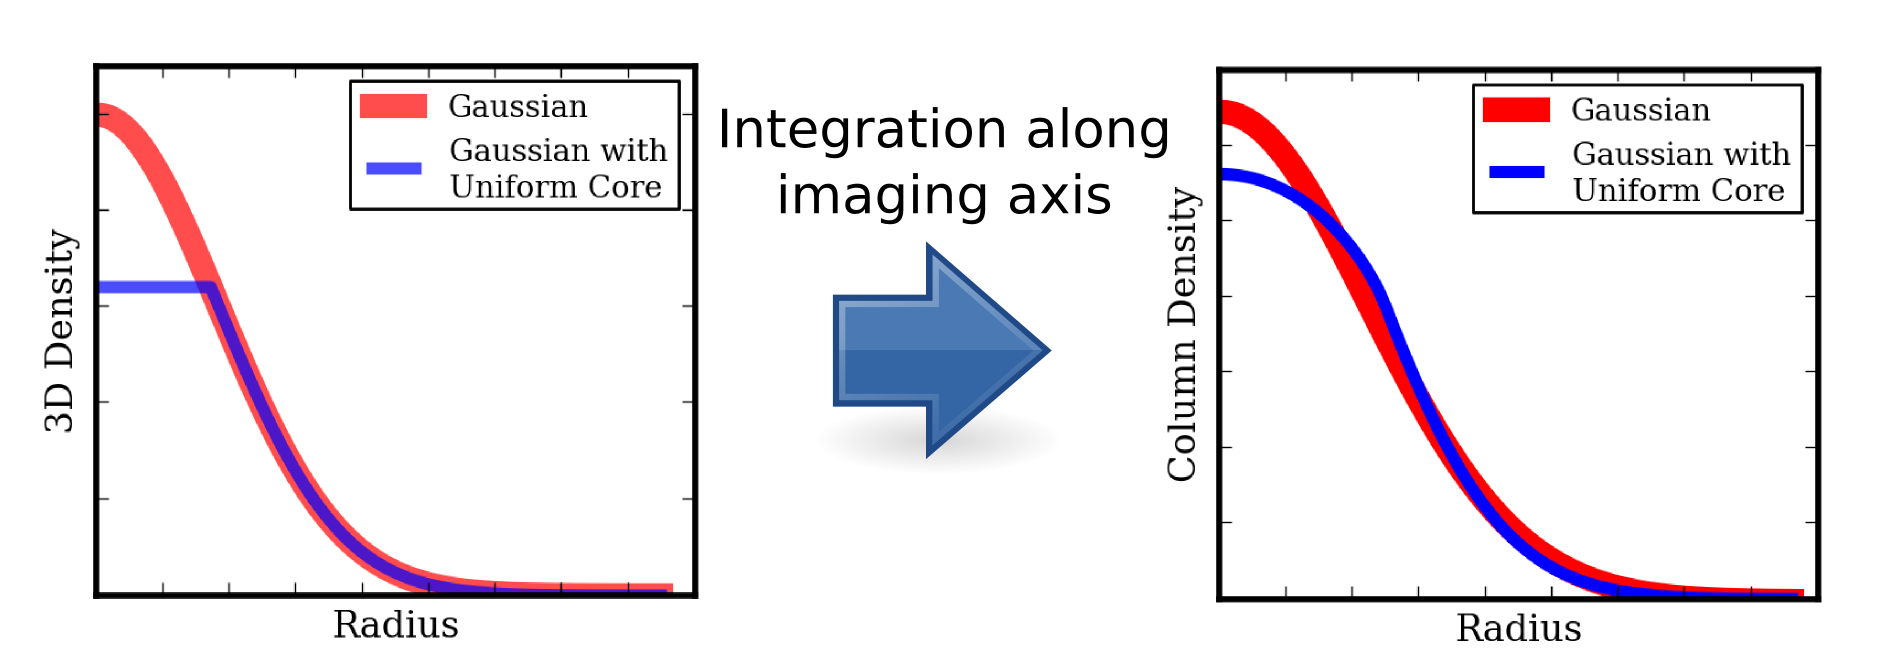
\includegraphics[width=0.85\textwidth]{../figures/mott/mott-fit-illustration.png}
\caption{\small Illustration of the Mott fit function which was implemented to
extract the central density from an \text{in-situ} measurement of the column
density.  }  
\label{fig:mott-fit-ill}
\end{figure}
In Fig.~\ref{fig:mott-fit-cloud}, a Gaussian fit to the column density is shown
as a red line, and the Mott fit is shown as a blue line.  It is clear that the
Mott fit provides a better representation of the observed profiles. 

We used the Mott fits to extract the central density of the cloud,
$\tilde{n}_{0}$ for various atom numbers and interaction strengths.  With our
knowledge of the trap parameters we calculated (within the LDA) profiles that
could be compared to the measurements.  The reader is reminded that, to realize
the LDA, one must have a solution for the homogeneous Hubbard model at a grid
of values for the Hubbard parameters $U/t$, $T/T$ and $\mu/t$. For example, in
Chapter~\ref{chap:compensated-optical-lattice} we used the HTSE to second
order as a solution for a homogeneous system to carry out the LDA.  For our
experiments, we find that, to reproduce the measured data, we had to realize
the calculations at a much lower temperature.  The validity of the HTSE breaks
down at around $T/t\approx 2.4$,  so we turned to a set of solutions using NLCE
and DQMC which were provided by our theory collaborators.   At the end of
Chapter~\ref{chap:hubbardmodel}, we have briefly described the NLCE and DQMC
techniques; refer to Appendix~\ref{app:numerical} for more details. 


In Fig.~\ref{fig:n0mott} we show the comparison between the experimental data
and the numerical calculations for the central density  at two different values
of the temperature $T/t_{0}$.  For the calculations, it is assumed that the
entire sample is in equilibrium at a temperature $T$.  The local value of $T/t$
then varies according to the variation of $t$ in our lattice.  \FigureThree
Figure~\ref{fig:n0mott} is very revealing.  First of all, it shows dramatically
the Mott insulating behavior obtained at large interaction strengths, where the
central density of the cloud does not depend much at all on atom number.
Secondly,  a clear Mott insulating behavior can be observed down to
$U_{0}/t_{0}=11.1$.   This is in contrast with previous observations of the
Mott insulating regime~\cite{Jordens2008,Schneider2008} which, due to samples
at larger temperatures ($T>t$), required significantly larger values of $U/t$
($U/t \geq 18$) to obtain evidence for an incompressible state.   

The intermediate values of $U_{0}/t_{0}$ ($\approx 11$) at which we can detect
Mott insulating behavior are revealing of the temperature of the sample,  which
by comparison with the numerical calculations shown in Fig.~\ref{fig:n0mott}
can be bounded to be $T/t_{0}<1$.  This value is consistent with the value that
was obtained using light-scattering thermometry, as will be explained later on
in Chapter~\ref{chap:afmbragg}.  

 
In addition to obtaining the central density from a fit to the column density
distribution, we also went ahead and analyzed the spatial dependency of the
column density profiles. One of the advantages of realizing the Hubbard model
with an external confinement potential is that the chemical potential varies
spatially and gives the opportunity to characterize multiple regimes within a
single cloud~\cite{Gemelke2009}. 

The compressibility as a function of density is an important indicator for the
formation of a Mott insulator.   A Mott insulating state is incompressible, and
occurs at a density $\tilde{n}=1$.  If one can measure compressibility as
a function of density then one can provide direct proof of having accessed the
Mott insulating regime.  
 
The isothermal compressibility of a gas is defined as 
\begin{equation}
    \kappa = \frac{1}{n^{2}} \frac{ \partial n }{ \partial \mu }. 
\end{equation} 
For atoms in a 3D lattice we consider the unitless quantity $(t/a^{3})\kappa$,
where $a$ is the lattice spacing.  In the limit of zero lattice depth,
$t\rightarrow - \frac{a}{2\pi} \int_{-\pi/a}^{\pi/a} \frac{\hbar^{2}q^{2}}{2m}
\exp[ i q a]\,\text{d}q = (2/\pi^{2}) E_{r}$, where $q$ is the quasimomentum,
$E_{r} = \frac{ \hbar^{2} \pi^{2}}{ 2ma^{2} } $ is the recoil energy, and $m$
is the mass of the particles.   For a non-interacting free gas, the
compressibility at zero temperature is given by $\kappa_{0} = \frac{
3}{2nE_{F}}$, where $E_{F}$ is the Fermi energy for each spin component. Here
we consider the normalized compressibility $\tilde{\kappa}$, defined as 
\begin{equation} 
\tilde{\kappa} \equiv  \frac{ (t/a^{3})\kappa  } 
                       {( 2E_{r} /(\pi^{2}a^{3})) \kappa_{0}} =  
             \frac{ (3\pi^{2})^{2/3} }{ 2 } 
             \frac{ \partial \tilde{n}^{2/3} }{ \partial (\mu/t) },
\end{equation}
where $\tilde{n} = a^{3}n$.

\FigureOne In Fig.~\ref{fig:fig1} we show results of numerical calculations for
$\tilde{\kappa}$ at various values of $T/t$ and $U/t$, obtained using
determinantal quantum Monte Carlo (DQMC)~\cite{PhysRevD.24.2278,Paiva2010}, a
numerical linked-cluster expansion (NLCE)~\cite{Rigol2006,Tang2013} up to the
eighth order in the site expansion, and a high temperature series expansion
(HTSE) up to second order in $T/t$~\cite{Henderson1992}.  These three methods
complement each other, and provide results over a wide range of interactions
and temperatures.  Figure~\ref{fig:fig1} shows that the calculated
compressibility diminishes at half-filling, as the system enters the Mott
insulating regime, and at $\tilde{n}=2$, where a band insulator forms. 


\FigureTwo The \textit{in-situ} column density measured in the experiment is
azimuthally averaged, and the inverse Abel transform\footnote{The inverse Abel
transform is a way to obtain the density profile from the column density
profile, assuming spherical symmetry of the sample. We perform the inverse Abel
transform with the filtered back-projection algorithm, as implemented in the
{scikit-image} image processing library~\cite{scikit-image}.}  is used to
obtain the density profile of the cloud.  Figure~\ref{fig:mottfig2} shows the
column density and density profiles for three different values of
$U_{0}/t_{0}$, compared with profiles obtained from numerical calculations for
our trap potential. For the calculations we set $T$ and the global chemical
potential, $\mu_{0}$; local values of $U/t$, $T/t$, and $\mu/t$ are then
calculated using the known trap potential.  As was explained above, the local
value of the density is obtained from linear interpolation between NLCE and
DQMC results for a homogeneous system calculated in a $(U/t,T/t,\mu/t)$ grid.  
 
We obtain $\tilde{\kappa}$ from the measured and calculated density profiles as 
\begin{equation}
\tilde{\kappa} =   
             \frac{ (3\pi^{2})^{2/3} }{ 2 } 
             \frac{ \partial \tilde{n}^{2/3} }{ \partial r } 
      \left(   \frac{ \partial (\mu/t) }{ \partial r }   \right)^{-1},
\end{equation}
where the spatial derivative of the local chemical potential is determined from
the trap parameters.  For the experimental data, the azimuthal average of the
column density, and the inverse Abel transform are noisy at small radii, so, to
avoid excessive noise in the determination of the radial derivative of
$\tilde{n}^{2/3}$, we restrict our analysis to $r/a > 12$.
Figure~\ref{fig:compr-mott} shows $\tilde{\kappa}$ vs $\tilde{n}$ for the
experimental data and for the calculated density profile.  The decrease of the
compressibility near $\tilde{n}\approx 1$, for $U_{0}/t_{0}=11.1$ and 14.5, is
consistent with the system entering the Mott insulating regime. 

\FigureFour

\section{Summary} 

The compressibility, shown in Fig.~\ref{fig:compr-mott}, and the central
density, shown in Fig.~\ref{fig:n0mott} are both consistent with the system
entering the Mott insulating regime for values of $U_{0}/t_{0} \geq 11.1$.
Qualitatively, we observe that in both cases the data is consistent with
$T/t_{0}<1$.   Below $T/t_{0}\approx1$, the density and the compressibility are
nearly insensitive to temperature, since most of the entropy in the system
resides in the spin degree of freedom.   

We have found in this analysis, that the systematic uncertainty in the trap
parameters prevents us from using the compressibility for a more precise
quantitative determination of temperature.   In the same system, a measurement
of AFM correlations using Bragg scattering of light showed $T/t_{0}=
0.58\pm0.07$ as will be explained in the next chapter. 

\section{Comparison to previous work} 


Previous ground-breaking experiments have investigated the Mott transition in
trapped lattice fermions by measuring the variation of the bulk double
occupancy with atom number~\cite{Jordens2008,Scarola2009,Jordens2010,Taie2012},
and the response of the cloud radius to changes in external
confinement~\cite{Schneider2008}, both of which are related to the global
compressibility, and are severely suppressed for large interactions.  Bulk
measurements, as in all previous fermionic Mott insulator experiments, present
the complication that they are an average over both metallic and insulating
phases simultaneously present in the trap.  In order to make the Mott
transition clearer, one would like to have access to the \textit{local}
compressibility, as we have shown here.  Access to the local compressibility
has enabled us to, for the first time, observe clear Mott plateaus (vs. atom
number Fig.~\ref{fig:n0mott} and vs. position/chemical potential
Fig.~\ref{fig:compr-mott}) in a cold gas of fermionic atoms.  

Furthermore, it is interesting to study the Mott insulating regime at
intermediate values of the coupling, where temperatures below the tunneling
energy are required to enter the Mott regime.  All previous work on fermionic
Mott insulators focused on strong interactions ($U/t>18$), where a Mott
insulator is robust even for $T>t$.  This regime is well understood by theory,
and can be benchmarked by simple numerical methods, such as the atomic
limit~\cite{Jordens2008} and the HTSE~\cite{Jordens2010,Taie2012}.   It was our
goal to explore the Mott insulating regime at intermediate coupling,  where the
system is in closer proximity to the antiferromagnetic phase transition due to
the fact that the N\'{e}el temperature is maximal there.   It is near this
coupling region where experiment can push theory to its limit.   In fact, the
numerical calculations developed with our theory collaborators over the course
of this work are the current state-of-the art for the 3D Hubbard model. 

The local compressibility, as demonstrated here, will be a useful tool to
characterize many-body phases in the 3D Hubbard away from half-filling at
temperatures less than the tunneling energy.   This regime,  analogous to the
pseudo-gap regime in high-$T_{c}$ materials, is of great interest as it is not
entirely understood by theory.  In addition, going into two-dimensions,  one
may find, in the local compressibility, signatures of phase separation and stripe
formation in the Hubbard model~\cite{PhysRevB.81.201101,PhysRevB.80.245102}. 


